\documentclass[11pt,a4]{article}
\usepackage{graphicx}
\usepackage{geometry}
\geometry{top=2.5cm,bottom=2.5cm,left=2.5cm,right=2.5cm}
\usepackage{amsmath}

\title{My Report LaTeX \LaTeX}
\author{Manosh T M}
\date{\today}




\begin{document}
\maketitle
\begin{abstract}
	The 2015 Africa Cup of Nations Final was a football match that took place on 8 February 2015 to determine the winner of the 2015 Africa Cup of Nations, the football championship of Africa organised by the Confederation of African Football (CAF). The match was held at the Estadio de Bata in Bata, Equatorial Guinea, and was contested by Ghana and Ivory Coast. Ghana reached the final by winning their qualifying group and then defeating Guinea and Equatorial Guinea in the quarter-final and semi-final. Ivory Coast also qualified as group winners, after which they beat Algeria and the Democratic Republic of the Congo.
\end{abstract}

\section{Introduction}
The 2015 Africa Cup of Nations Final was a football match that took place on 8 February 2015 to determine the winner of the 2015 Africa Cup of Nations, the football championship of Africa organised by the Confederation of African Football (CAF). The match was held at the Estadio de Bata in Bata, Equatorial Guinea, and was contested by Ghana and Ivory Coast. Ghana reached the final by winning their qualifying group and then defeating Guinea and Equatorial Guinea in the quarter-final and semi-final. Ivory Coast also qualified as group winners, after which they beat Algeria and the Democratic Republic of the Congo.

\section*{Football}
The 2015 Africa Cup of Nations Final was a football match that took place on 8 February 2015 to determine the winner of the 2015 Africa Cup of Nations, the football championship of Africa organised by the Confederation of African Football (CAF). The match was held at the Estadio de Bata in Bata, Equatorial Guinea, and was contested by Ghana and Ivory Coast. Ghana reached the final by winning their qualifying group and then defeating Guinea and Equatorial Guinea in the quarter-final and semi-final. Ivory Coast also qualified as group winners, after which they beat Algeria and the Democratic Republic of the Congo.

\begin{equation}
\frac{\partial y}{\partial t}=\oint\alpha\beta\sqrt{x^2+y^2} dx
\label{My_eq}
\end{equation}

\begin{equation}
F=am
\label{Eq:1}
\end{equation}


The 2015 Africa Cup of Nations Final was a football match that took place on 8 February 2015 to determine the winner of the 2015 Africa Cup of Nations, the football championship of Africa organised by the Confederation of African Football (CAF). The match was held at the Estadio de Bata in Bata, Equatorial Guinea, and was contested by Ghana and Ivory Coast. Ghana reached the final by winning their qualifying group and then defeating Guinea and Equatorial Guinea in the quarter-final and semi-final. Ivory Coast also qualified as group winners, after which they beat Algeria and the Democratic Republic of the Congo. Equation (\ref{Eq:1})

\begin{equation}
G_{\mu \nu }=R_{\mu \nu }-{\frac {1}{2}}Rg_{\mu \nu }
\end{equation}

The match was held at the Estadio de Bata in Bata, Equatorial Guinea, and was contested by Ghana and Ivory Coast.\\

Ghana reached the final by winning their qualifying group and then defeating Guinea and Equatorial Guinea in the quarter-final and semi-final. Ivory Coast also qualified as group winners, after which they beat Algeria and the Democratic Republic of the Congo. Equation (\ref{Eq:1})

\begin{figure}[h]
	\centering
	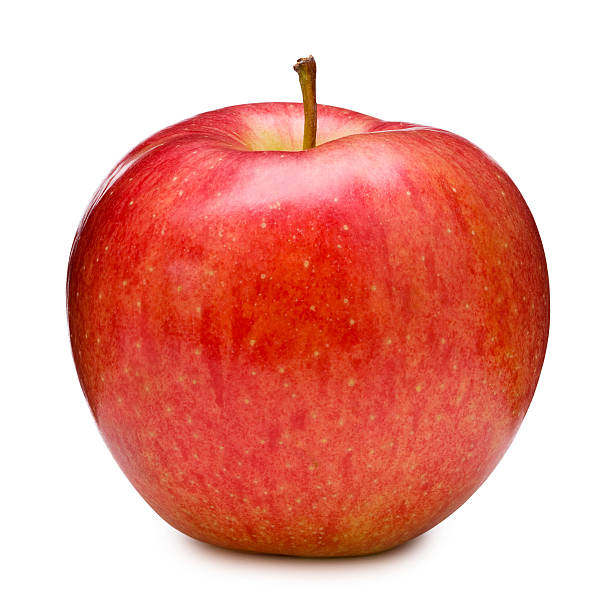
\includegraphics[width=5cm]{images/fig1}
	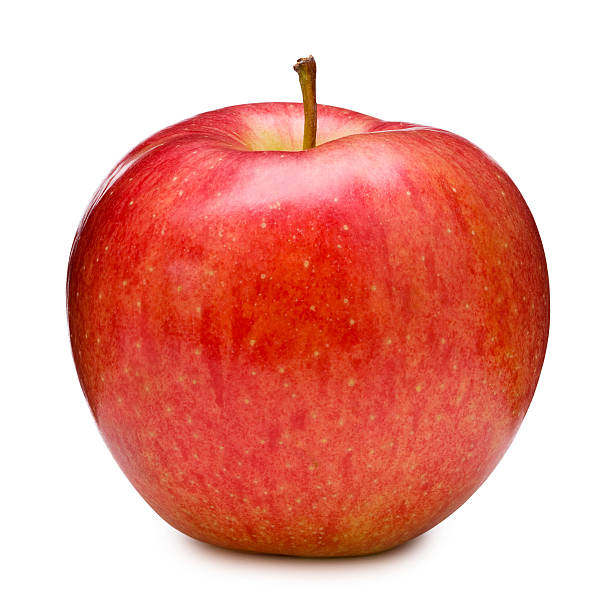
\includegraphics[width=5cm]{images/fig1}
	\caption{My first image}
	\label{fig:1}
\end{figure}


\begin{table}[h]
	\begin{center}
		\begin{tabular}{|c|c|r|c|}
			\hline
			\rule[-1ex]{0pt}{2.5ex} Name & Place & Age & Remarks \\
			\hline
			\rule[-1ex]{0pt}{2.5ex} Appu & EKM & 12 &  \\
			\hline
			\rule[-1ex]{0pt}{2.5ex} Ammu & TVM & 13 &  \\
			\hline
			\rule[-1ex]{0pt}{2.5ex} Hari & USA &12  &  \\
			\hline
			\rule[-1ex]{0pt}{2.5ex} Basi & JAP  & 7 &  \\
			\hline
			\rule[-1ex]{0pt}{2.5ex} Athul & PLUTO & 20 &  \\
			\hline
		\end{tabular}
	\end{center}
\caption{My table}
\label{tab:1}
\end{table}


Ghana reached the final by winning their qualifying group and then defeating Guinea and Equatorial Guinea in the quarter-final and semi-final. Ivory Coast also qualified as group winners, after which they beat Algeria and the Democratic Republic of the Congo. Equation (\ref{Eq:1})
\subsection{Apple}
Ghana reached the final by winning their qualifying group and then defeating Guinea and Equatorial Guinea in the quarter-final and semi-final. Ivory Coast also qualified as group winners, after which they beat Algeria and the Democratic Republic of the Congo. Equation (\ref{Eq:1})Ghana reached the final by winning their qualifying group and then defeating Guinea and Equatorial Guinea in the quarter-final and semi-final. Ivory Coast also qualified as group winners, after which they beat Algeria and the Democratic Republic of the Congo. Equation (\ref{Eq:1}) Table (\ref{tab:1})




\section{Main content}

\subsection{Apple}
Ghana reached the final by winning their qualifying group and then defeating Guinea and Equatorial Guinea in the quarter-final and semi-final. Ivory Coast also qualified as group winners, after which they beat Algeria and the Democratic Republic of the Congo. Equation (\ref{Eq:1})Ghana reached the final by winning their qualifying group and then defeating Guinea and Equatorial Guinea in the quarter-final and semi-final. Ivory Coast also qualified as group winners, after which they beat Algeria and the Democratic Republic of the Congo. Equation (\ref{Eq:1}) Table (\ref{tab:1})

\end{document}